% scenario de presentation des éléments

\def\schemaScenarioPresentation{%
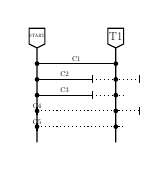
\begin{tikzpicture}[scale=0.1]%
\def\date{0};%
\def\contraintName{C1};%
\def\ypos{-2};%
\def\min{10};%
\def\nom{10};%
\def\max{10};%
\fill (\date,\ypos) circle (0.3);%
\fill (\date+\nom,\ypos) circle (0.3);%
\draw (\date,\ypos) -- ++(\min,0) node[midway,above,scale=0.25] {\contraintName};%
\draw (\date+\min,\ypos+0.5) -- ++(0,-1);%
\draw[densely dotted] (\date+\min,\ypos) -- (\date+\max,\ypos);%
\draw (\date+\max,\ypos+0.5) -- ++(0,-1);%
%
\def\contraintName{C2};%
\def\ypos{-4};%
\def\min{7};%
\def\nom{10};%
\def\max{13};%
\fill (\date,\ypos) circle (0.3);%
\fill (\date+\nom,\ypos) circle (0.3);%
\draw (\date,\ypos) -- ++(\min,0) node[midway,above,scale=0.25] {\contraintName};%
\draw (\date+\min,\ypos+0.5) -- ++(0,-1);%
\draw[densely dotted] (\date+\min,\ypos) -- (\date+\max,\ypos);%
\draw (\date+\max,\ypos+0.5) -- ++(0,-1);%
%
\def\contraintName{C3};%
\def\ypos{-6};%
\def\min{7};%
\def\nom{10};%
\def\max{11};%
\fill (\date,\ypos) circle (0.3);%
\fill (\date+\nom,\ypos) circle (0.3);%
\draw (\date,\ypos) -- ++(\min,0) node[midway,above,scale=0.25] {\contraintName};%
\draw (\date+\min,\ypos+0.5) -- ++(0,-1);%
\draw[densely dotted] (\date+\min,\ypos) -- (\date+\max,\ypos);%
\def\contraintName{C4};%
\def\ypos{-8};%
\def\min{0};%
\def\nom{10};%
\def\max{13};%
\fill (\date,\ypos) circle (0.3);%
\fill (\date+\nom,\ypos) circle (0.3);%
\draw (\date,\ypos) -- ++(\min,0) node[midway,above,scale=0.25] {\contraintName};%
\draw (\date+\min,\ypos+0.5) -- ++(0,-1);%
\draw[densely dotted] (\date+\min,\ypos) -- (\date+\max,\ypos);%
\draw (\date+\max,\ypos+0.5) -- ++(0,-1);%
%
\def\contraintName{C5};%
\def\ypos{-10};%
\def\min{0};%
\def\nom{10};%
\def\max{11};%
\fill (\date,\ypos) circle (0.3);%
\fill (\date+\nom,\ypos) circle (0.3);%
\draw (\date,\ypos) -- ++(\min,0) node[midway,above,scale=0.25] {\contraintName};%
\draw (\date+\min,\ypos+0.5) -- ++(0,-1);%
\draw[densely dotted] (\date+\min,\ypos) -- (\date+\max,\ypos);%
\def\nodeName{START};%
\def\ypos{-12};%
\draw (\date,0) -- ++(-1,0.5) -- ++(0,2) -- ++(2,0) -- ++(0,-2) -- ++(-1,-0.5) -- (\date, \ypos);%
\draw (\date,1.5) node[scale=0.17]{\nodeName};%
%
\def\date{10};%
\def\nodeName{\Huge T1};%
\def\ypos{-12};%
\draw (\date,0) -- ++(-1,0.5) -- ++(0,2) -- ++(2,0) -- ++(0,-2) -- ++(-1,-0.5) -- (\date, \ypos);%
\draw (\date,1.5) node[scale=0.17]{\nodeName};%
%
\end{tikzpicture}%
}